\documentclass[dvisvgm,tikz,border=4pt]{standalone}\usepackage{amsmath,amssymb}
\usetikzlibrary{arrows.meta,decorations.markings,backgrounds,cd,calc}
\colorlet{c1}{blue!70!black}\colorlet{c2}{red!70!black}\colorlet{c3}{green!45!black}
\tikzset{
 ->-/.style={decoration={markings,mark=at position .55 with {\arrow{Stealth[length=2.4mm]}}},postaction={decorate}},
 ->>-/.style={decoration={markings,mark=at position .5 with {\arrow{Stealth[length=2.4mm]}},mark=at position .6 with {\arrow{Stealth[length=2.4mm]}}},postaction={decorate}},
 every picture/.append style={show background rectangle, background rectangle/.style={fill=white}}
}

\begin{document}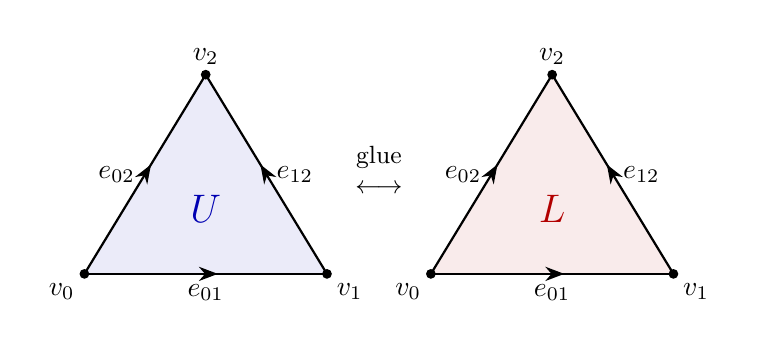
\begin{tikzpicture}[scale=1.1]
\foreach \s/\n/\col in {0/U/c1,4/L/c2}{
\begin{scope}[xshift=\s cm]
\coordinate (A) at (0,0); \coordinate (B) at (2.8,0); \coordinate (C) at (1.4,2.3);
\fill[\col!8] (A)--(B)--(C)--cycle;
\draw[thick,->-] (A)--(B) node[midway,below]{$e_{01}$};
\draw[thick,->-] (B)--(C) node[midway,right]{$e_{12}$};
\draw[thick,->-] (A)--(C) node[midway,left]{$e_{02}$};
\foreach \p/\m/\pos in {A/v_0/below left,B/v_1/below right,C/v_2/above}{\fill (\p) circle(1.6pt) node[\pos]{$\m$};}
\node[\col,font=\Large] at (1.4,0.75){$\n$};
\end{scope}}
\node[align=center,font=\small] at (3.4,1.2){glue\\$\longleftrightarrow$};
\end{tikzpicture}\end{document}
